
	\documentclass{article}
	\usepackage{amsmath,amssymb}
	\usepackage[inline]{enumitem}
	\usepackage{blindtext}
	\usepackage{booktabs}
	\usepackage{graphicx}
	\usepackage{xcolor}
	\usepackage[vmargin = 1.5in, top = 1in, bottom = 1.2in, letterpaper]{geometry}
	\usepackage{listings}
	\usepackage{courier}
	\usepackage{multicol}
	\usepackage{multirow}
	\usepackage{bm}
	\usepackage{algorithm}
	\usepackage{algpseudocode}
	\lstset{
	basicstyle = \small\tt,
	keywordstyle = \ttfamily\bfseries\color{blue},
	commentstyle = \it\color[cmyk]{1,0,1,0},
	stringstyle = \tt\color[RGB]{128,0,0},
	%frame = single,
	backgroundcolor = \color[RGB]{245,245,244},
	breaklines,
	extendedchars = false,
	xleftmargin = 2em,
	xrightmargin = 2em,
	aboveskip = 1em,
	tabsize = 4,
	showspaces = false
	showstringspaces = false
	}
	\begin{document}
	
	% \newfontfamily\courier{Courier New}

	
	\title{STAT 580 Homework 2}
	\author{Yifan Zhu}
	\maketitle
	
	\begin{enumerate}[leftmargin = 0 em, label = \arabic*., font = \bfseries]
	\item 
	\lstinputlisting[language = C]{./Codes/p1.c}

	
	\item 
	\begin{enumerate}
		\item 
		$\int_{1}^{10} f(x) = 1 \Rightarrow c \int_{1}^{10} \frac{1}{x} \mathrm{d}x= c (\log 10 - 0) = 1 \Rightarrow \frac{1}{\log 10}$. Hence
		\[F(x) = \int_{1}^x f(x) \mathrm{d}x = \int_{1}^x \frac{1}{\log 10} \frac{1}{x} \mathrm{d}x = \frac{\log x}{\log 10} = \log_{10} (x) ,\, 1 < x < 10\]

		Hence the inverse function
		\[F^{-1}(u) = 10^u,\, 0<u<1\]

		Thus the algorithm would be
		\begin{algorithm}
			\caption{Sampling $X$ with cdf $F(x) = \log_{10}(x)$}
			\begin{algorithmic}[1]
				\State Generate $U \sim Unif(0,1)$;
				\State Set $X = 10^U$;
			\end{algorithmic}
		\end{algorithm}

		\item 

		\ 

		\lstinputlisting[language = C]{./Codes/p2.c}

		\item 

		\ 
		
		\lstinputlisting[language = R]{./Codes/p2.R}
		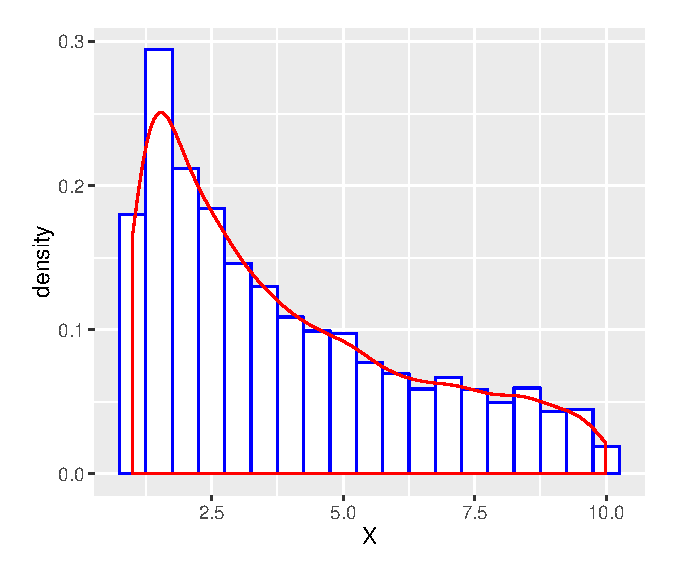
\includegraphics[width = 0.8\textwidth]{p2density.eps}

	\end{enumerate}

	\item 
	\begin{enumerate}
		\item 
		\lstinputlisting[language = R]{./Codes/p3.R}

		The density when using $g_1 (x) = \mathrm{e}^{-x}$:

		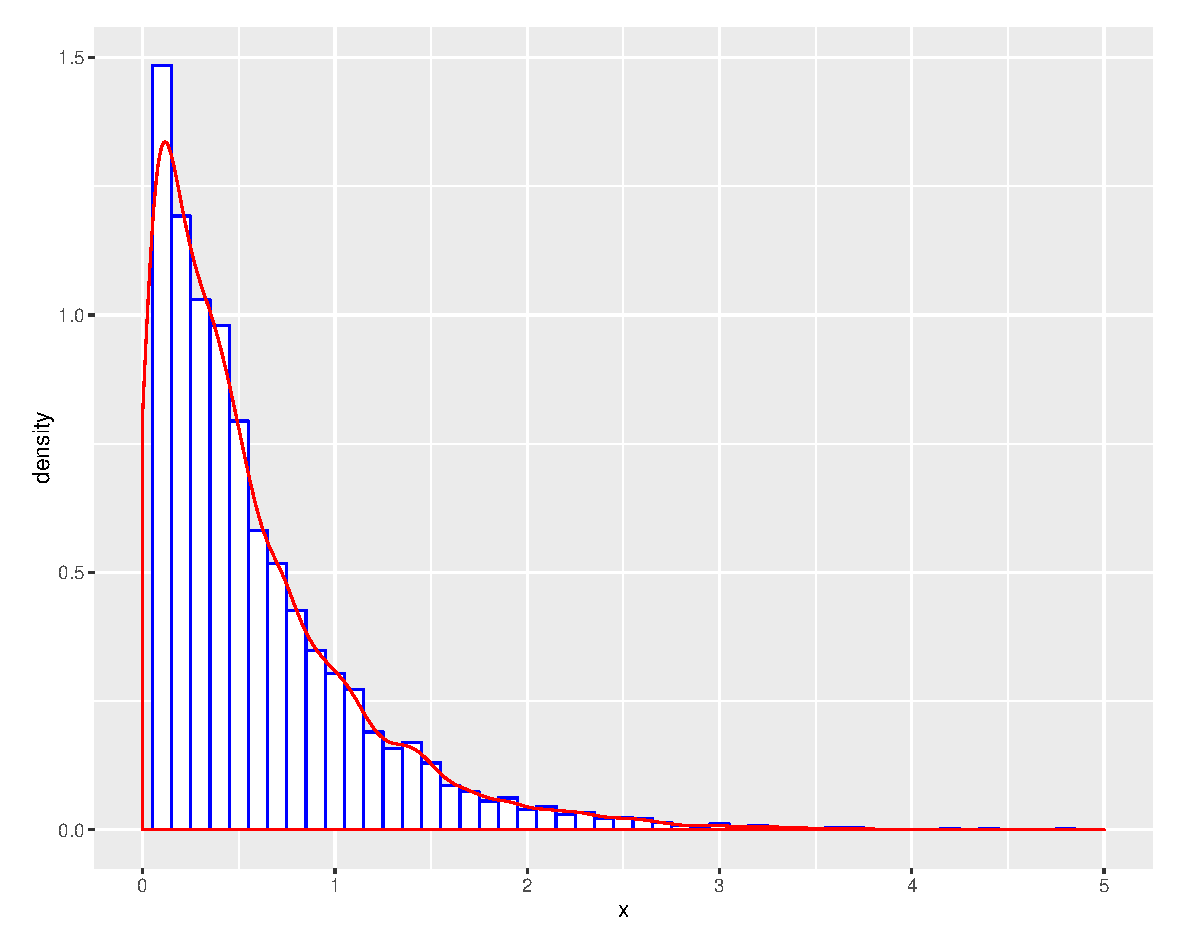
\includegraphics[width = 0.8\textwidth]{p3sample1.eps}

		The density when using $g_2 (x) = \frac{\pi (1 + x^2)}{2}$:

		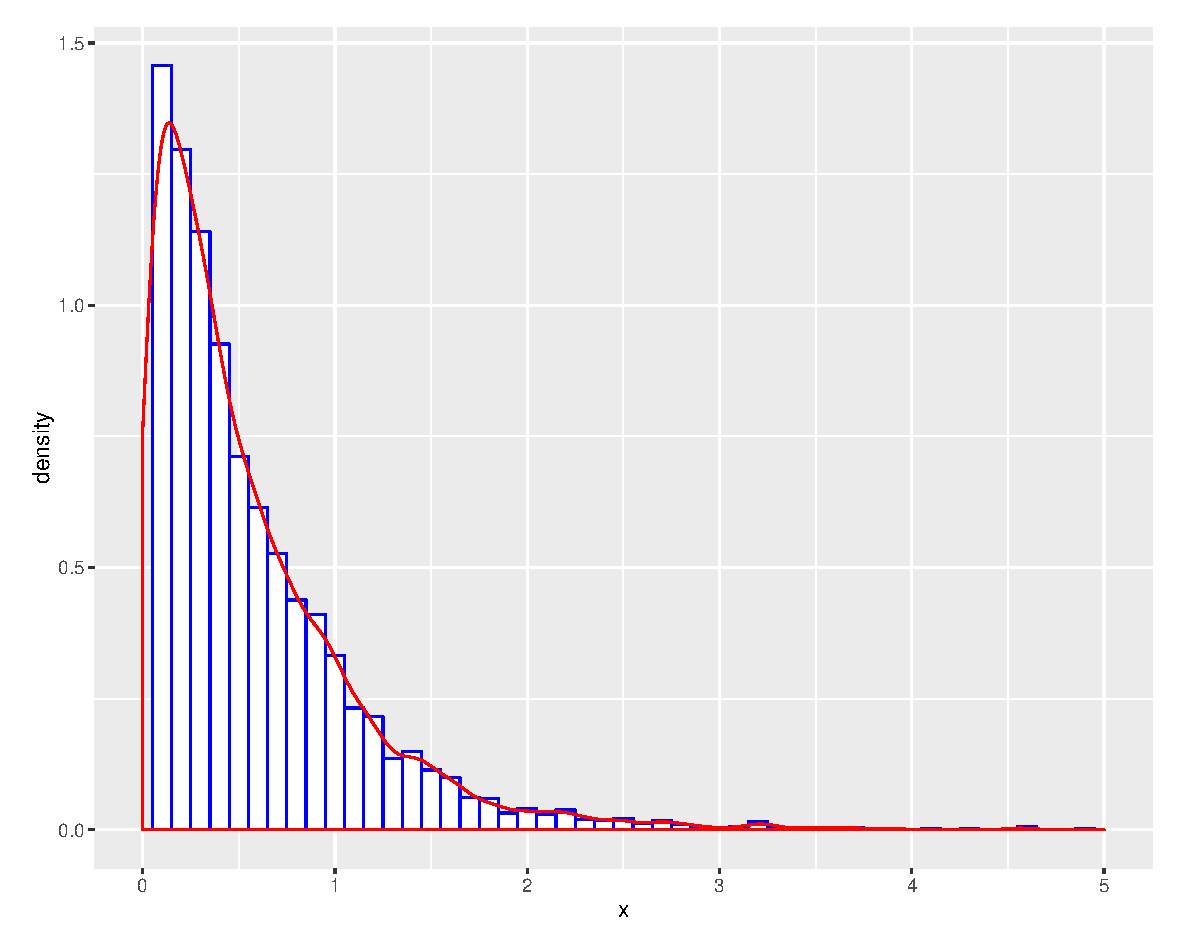
\includegraphics[width = 0.8\textwidth]{p3sample2.eps}

		\item

		The density we get using $g_1$ and $g_2$ are almost the same. And the time using $g_2$ is longer than the time using $g_1$. 

		The \verb|system.time(sample1(5000))| returns the time when using $g_1$:
		\begin{verbatim}
user  system elapsed 
0.04    0.00    0.04 
		\end{verbatim}

		The \verb|system.time(sample2(5000))| returns the time when using $g_2$:
		\begin{verbatim}
user  system elapsed 
0.07    0.00    0.08 
		\end{verbatim}
	\end{enumerate}
	
	\item 

	\

	\begin{algorithm}
		\caption{Sampling from $f(x,y) \propto x^{\alpha}y$ with support being $x^2 + y^2 \leq 1$ in the first quadrant}
		\begin{algorithmic}[1]
			\State  Generate $X \sim Beta(\alpha + 1, 1)$ and $Y \sim Beta(2,1)$ independently;
			\If {$X^2 + Y^2 > 1$} \Statex {Go to Step 1;} \Else \Statex Return $(X,Y)$;\EndIf
		\end{algorithmic}
	\end{algorithm}
	

 	\end{enumerate}



	\end{document}